% !TeX root = hw_1-koncni_avtomati.tex
\documentclass{article}

\usepackage{graphicx}
\usepackage{tikz}
\usepackage{parskip}
\usetikzlibrary {arrows.meta,automata,positioning}
\title{Algoritmi v bioinformatiki - 1. Domača naloga}
\author{Jan Panjan}
\date{\today}

\begin{document}

\tikzset{
node distance=2.6cm, % specifies the minimum distance between two nodes. Change if necessary.
every state/.style={thick, fill=gray!10}, % sets the properties for each ’state’ node
->, % makes the edges directed
>={Stealth} % make arrow heads bold
}

\maketitle
\newpage

\begin{enumerate}
	\item \textit{Konstruirajte deterministični končni avtomat, ki v mRNK materialu prepozna
		zaključne kodone.}
		\begin{enumerate}
			\item Grafično:

				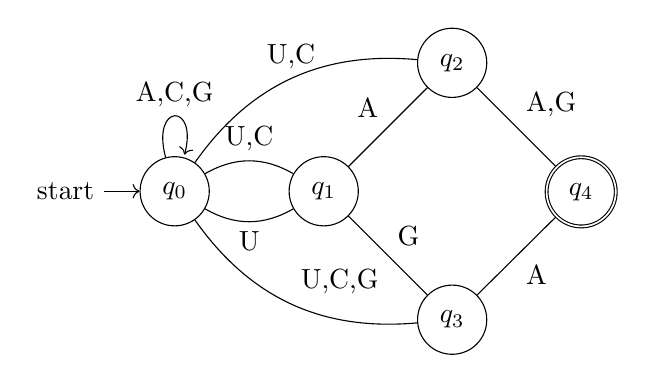
\begin{tikzpicture}
					\node[state, initial]   (q0)                     {$q_0$};
					\node[state] 			(q1) [right=of q0]       {$q_1$};
					\node[state] 	        (q2) [above right=of q1] {$q_2$};
					\node[state] 		    (q3) [below right=of q1] {$q_3$};
					\node[state, accepting] (q4) [below right=of q2] {$q_4$};

					\draw (q0) edge[loop above, above]       node{A,C,G}        (q0)
						(q0) edge[below, bend right]       node{U}        (q1)
						(q1) edge[above left]  node{A}        (q2)
						(q1) edge[above, bend right]  node{U,C}        (q0)
						(q1) edge[above right]  node{G}        (q3)
						(q2) edge[above right] node{A,G}      (q4)
						(q2) edge[above, bend right] node{U,C}      (q0)
						(q3) edge[below right] node{A}        (q4)
						(q3) edge[above right, bend left] node{U,C,G}        (q0);
				\end{tikzpicture}
				\newline

			\item S formalnim opisom peterike $\left[ \Sigma, Q, q_0, F, \delta \right]$:

				\begin{itemize}
					\item $\Sigma = \{ A, U, C, G \}$
					\item $Q = \{ q_1, q_2, q_3, q_4 \}$
					\item $q_0 = q_0$
					\item $F = \{ q_4 \}$
					\item \begin{tabular}{|c||c|c|c|c|}
							\hline
							$\delta$ & A & U & C & G \\
							\hline \hline
							0 & $q_0$ & $q_1$ & $q_0$ & $q_0$\\
							\hline
							1 & $q_2$ & $q_0$ & $q_0$ & $q_3$\\
							\hline
							2 & $q_4$ & $q_0$ & $q_0$ & $q_4$\\
							\hline
							3 & $q_4$ & $q_0$ & $q_0$ & $q_0$\\
							\hline
							4 & / & / & / & / \\
							\hline
						\end{tabular}
				\end{itemize}
		\end{enumerate}

		\newpage

	\item \textit{Kako se rešitev 1. naloge spremeni, če želimo s pomočjo končnega
			avtomata poiskati vse pojavitve zaključnih kodonov? Zapišite algoritem
			in ponazorite njegovo delovanje na delu mRNK AUAUAAUGCUUGA. Koliko
		zaključnih kodonov vsebuje dani mRNK?}

		Njegovo končno stanje se spremeni, tako da ponovno začne iskati vzorec, ko
		pride enkrat do
		končnega stanja. To je vidno grafično kot povezava od $q_4$ do $q_0$ in
		spremenjene vrednosti v zadnji vrstici $\delta-$tabele.

		\begin{enumerate}
			\item Grafično:

				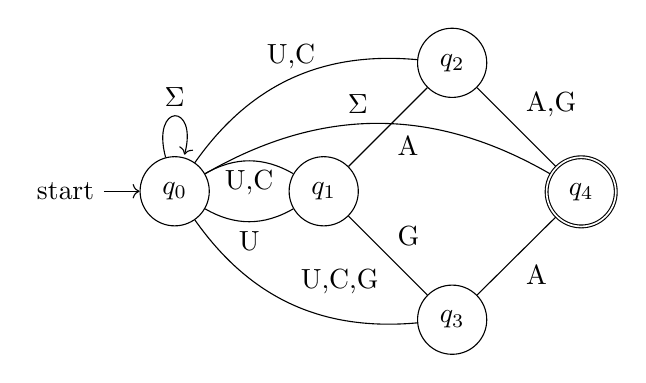
\begin{tikzpicture}
					\node[state, initial]   (q0)                     {$q_0$};
					\node[state] 			(q1) [right=of q0]       {$q_1$};
					\node[state] 	        (q2) [above right=of q1] {$q_2$};
					\node[state] 		    (q3) [below right=of q1] {$q_3$};
					\node[state, accepting] (q4) [below right=of q2] {$q_4$};

					\draw (q0) edge[loop above, above]       node{$\Sigma$}        (q0)
						(q0) edge[below, bend right]       node{U}        (q1)
						(q1) edge[below right]  node{A}        (q2)
						(q1) edge[below, bend right]  node{U,C}        (q0)
						(q1) edge[above right]  node{G}        (q3)
						(q2) edge[above right] node{A,G}      (q4)
						(q2) edge[above, bend right] node{U,C}      (q0)
						(q3) edge[below right] node{A}        (q4)
						(q3) edge[above right, bend left] node{U,C,G}        (q0)
						(q4) edge[above left, bend right] node{$\Sigma$}        (q0);
				\end{tikzpicture}

			\item S formalnim opisom peterike $\left[ \Sigma, Q, q_0, F, \delta \right]$:

				\begin{itemize}
					\item $\Sigma = \{ A, U, C, G \}$
					\item $Q = \{ q_1, q_2, q_3, q_4 \}$
					\item $q_0 = q_0$
					\item $F = \{ q_4 \}$
					\item \begin{tabular}{|c||c|c|c|c|}
							\hline
							$\delta$ & A & U & C & G \\
							\hline \hline
							0 & $q_0$ & $q_1$ & $q_0$ & $q_0$\\
							\hline
							1 & $q_2$ & $q_0$ & $q_0$ & $q_3$\\
							\hline
							2 & $q_4$ & $q_0$ & $q_0$ & $q_4$\\
							\hline
							3 & $q_4$ & $q_0$ & $q_0$ & $q_0$\\
							\hline
							4 & $q_0$ & $q_0$ & $q_0$ & $q_0$ \\
							\hline
						\end{tabular}
				\end{itemize}
		\end{enumerate}

		\newpage

		\textbf{Algoritem za iskanje STOP kodonov v mRNA vzorcu:} algoritem za izgradnjo
		$\delta-$tabele smo podali na vajah in ga ne bom ponovno napisal.
		Predpostavljam torej, da je tabela za naš končni avtomat že izgrajena.
		Iskanje vzorca v besedilu AUAUAAUGCUUGA poteka tako:

		\begin{tabular}{c|c c c c c c c c c c c c c}
			$q$ & 0 & 1 & 2 & 0 & 0 &  & & & & & & & \\
			$l$ & A & U & A & U & A & A & U & G & C & U & U & G & A \\
		\end{tabular}
\end{enumerate}

\end{document}
